\chapter{Gourmet Photography Dataset ed esperimenti}
\label{GPD}

\section{Contenuto e sviluppo di GPD}
Il Gourmet Photography Dataset \cite{sheng2021learning} è stato la base su cui sono stati sviluppati e sperimentati diversi algoritmi per l'estrazione delle feature al fine di studiare l'estetica delle  24000 immagini di cibo che lo compongono. Le fotografie vengono classificate in maniera binaria in base alla loro estetica, quindi le due classi sono rispettivamente:
\begin{itemize}
  \item \textbf{Classe positiva}, la quale contiene 13088 immagini 
  \item \textbf{Classe negativa}, la quale contiene 10912 immagini 
\end{itemize}

In Figura \ref{negativeGPD} e Figura \ref{positiveGPD} sono riportati alcuni esempi delle immagini contenute nel GPD per ognuna delle due classi.

\begin{figure}[H]
\centering
\includegraphics[height=40mm]{images/GPD/neg_111.jpg}
\quad
\includegraphics[height=40mm]{images/GPD/neg_544.jpg}
\quad
\vspace{5mm}
\includegraphics[height=40mm]{images/GPD/neg_1577.jpg}\\
\quad
\includegraphics[height=40mm]{images/GPD/neg_1800.jpg}
\quad
\vspace{5mm}
\includegraphics[height=40mm]{images/GPD/neg_2547.jpg}
\quad
\includegraphics[height=40mm]{images/GPD/neg_6158.jpg}
\quad
\includegraphics[height=40mm]{images/GPD/neg_2601.jpg}
\quad
\vspace{5mm}
\includegraphics[height=40mm]{images/GPD/neg_7650.jpg}
\quad
\includegraphics[height=40mm]{images/GPD/neg_9488.jpg}
\caption{Esempio di alcune immagini del GPD che a cui è associata la label negativa}
\label{negativeGPD}
\end{figure}

\begin{figure}[H]
\centering
\includegraphics[height=40mm]{images/GPD/pos_619.jpg}
\quad
\includegraphics[height=40mm]{images/GPD/pos_639.jpg}
\quad
\vspace{5mm}
\includegraphics[height=40mm]{images/GPD/pos_1008.jpg}\\
\quad
\includegraphics[height=40mm]{images/GPD/pos_1016.jpg}
\quad
\vspace{5mm}
\includegraphics[height=40mm]{images/GPD/pos_4061.jpg}
\quad
\includegraphics[height=40mm]{images/GPD/pos_4256.jpg}\\
\quad
\includegraphics[height=40mm]{images/GPD/pos_6183.jpg}
\quad
\vspace{5mm}
\includegraphics[height=40mm]{images/GPD/pos_6559.jpg}
\quad
\includegraphics[height=40mm]{images/GPD/pos_8218.jpg}
\caption{Esempio di alcune immagini del GPD che a cui è associata la label positiva}
\label{positiveGPD}
\end{figure}
%In Figura \ref{positiveGPD} e Figura \ref{negativeGPD} sono riportati alcuni esempi delle immagini contenute nel Gourmet Photography Dataset.

Inoltre questo dataset relativo alla valutazione estetica applicata alle immagini di cibo è stato il primo grande insieme di immagini che unissero la valutazione estetica all'ambito del cibo, in quanto in precedenza erano presenti in letteratura dataset di cibo e delle valutazioni delle prestazioni relative alla classificazione dei vari cibi, ma non c'erano dataset relativi alle due tematiche insieme.

Per creare il GPD sono state necessarie 3 fasi:
\begin{enumerate}
	\item \textbf{Raccolta delle immagini}, in modo tale che siano il più varie possibile sia nel contenuto che nelle condizioni di luminosità e colori, scartando le immagini duplicate e svolgendo un pre-processing che elimini bordi inutili e ruoti correttamente le immagini.
	\item \textbf{Scrittura delle label corrispondenti}, considerando il problema dell'estetica come un problema di tipo binario. Si hanno N coppie \{I$_{i}$,\^{y$_{i}$}\}$^{N}_{i=1}$, dove \^{y$_{i}$}$\in$\{0,1\} è la label associata all'immagine i-esima I$_{i}$ e N indica la numerosità delle immagini, in questo caso pari a 24000. Le immagini sono state valutate da 57 lavoratori del AMT (Amazon’s Mechanical Turk), i quali hanno avuto anche la possibilità di non esprimere un giudizio sulle immagini che secondo loro erano ambigue, poiché è necessario che le label risultanti da questo passaggio siano significative. In particolare quando un'immagine viene saltata tre volte essa viene automaticamente scartata e non viene più riproposta ad altri utenti. Uno schema del procedimento di valutazione appena illustrato è visibile in Figura \ref{pipeline}.
\begin{figure}[H]
\centering
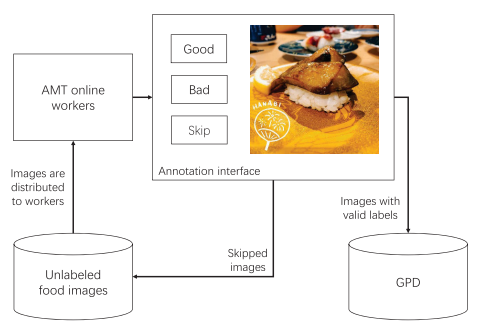
\includegraphics[scale=0.95]{images/pipeline.png}\caption{Schema tratto dal lavoro originale \cite{sheng2021learning} che illustra la pipeline della valutazione delle immagini del GPD da parte di 57 lavoratori del AMT (Amazon’s Mechanical Turk)}
\label{pipeline}
\end{figure}
	\item \textbf{Approvazione delle label da parte di otto fotografi esperti}, se almeno quattro di essi sono d'accordo con la label assegnata dagli utenti allora essa viene mantenuta, altrimenti la label è considerata ambigua e l'immagine viene eliminata.
\end{enumerate}
Le immagini verranno poi divise in modo randomico in:
\begin{itemize}
  \item \textbf{Training set}: 21600 immagini, di cui 
  \begin{itemize}
  \item 11779 positive
  \item 9821 negative
  \end{itemize}
  \item \textbf{Test set}: 10912 immagini, di cui
  \begin{itemize}
  \item 1309 positive
  \item 1091 negative
  \end{itemize}
\end{itemize}

\section{Test e risultati}
Nel lavoro originale \cite{sheng2021learning}, sono state provate varie combinazioni di feature e classificatore SVM (Support Vector Machine) con risultati di accuratezza sul test set abbastanza bassi, come è visibile nella prima parte della Tabella \ref{tabella_GPD}. In particolare le combinazioni sono le seguenti:
\begin{itemize}
\item \textbf{SVM e colore.} Il colore è una caratteristica molto significativa quando si parla di estetica, in questo caso il colore è stato codificato come un istogramma con 128 bin per i canali RGB. Inoltre i valori sono stati normalizzati rispetto alla media e alla varianza come segue:
\begin{equation} 
\label{normalizzazione}
x^{'}=\frac{x-\mu}{\sigma}
\end{equation}
In particolare $\mu$ indica la media, $\sigma$ indica la varianza e $x^{'}$ indica il valore $x$ a cui è stata applicata la normalizzazione.
\item \textbf{SVM e feature GIST.} Queste feature sono di tipo globale, in particolare viene estratto un array di feature con lunghezza pari a 512 partendo da una immagine a livelli di grigio di dimensione pari a 256x256. 
Anche in questo caso i valori sono stati normalizzati rispetto alla media e alla varianza come indicato al punto precedente in Formula ({\ref{normalizzazione}}).
\item \textbf{SVM e feature VGG.} Viene estratto un array di feature con lunghezza pari a 4096 dal penultimo layer di una rete VGG-16. In questo caso sono stati usati tre diversi modelli con contenuto semantico differente: VGG-objects, VGG-scenes e VGG-foods.
\end{itemize}
% cross entropy loss https://towardsdatascience.com/cross-entropy-loss-function-f38c4ec8643e
L'accuratezza cresce utilizzando delle reti neurali convoluzionali supervisionate, inizializzate con il dataset ImageNet \cite{deng2009imagenet} e utilizzando la cross-entropy per minimizzare la perdita e ottimizzare il modello. Nel training vengono utilizzate immagini scalate rispetto al lato più corto, tagliate e specchiate orizzontalmente in modo casuale al fine di aumentare il dataset disponibile.

\begin{table}[H]
\centering
\begin{tabular}{| c  c  c |}
\hline
Solution & Training Set & Test Set \\ [0.5ex]
\hline
%\textbf{SVM classifier} &  &  \\ [0.5ex]
\multicolumn{3}{|c|}{\textbf{SVM classifier}} \\ [0.5ex]
\hline
SVM + color & 72.4 & 63.3 \\
SVM + GIST & 78.1 & 64.4 \\
SVM + VGG-object & 90.8 & 74.7 \\
SVM + VGG-scenes & 86.8 & 72.4 \\
SVM + VGG-foods & 90.4 & 74.1 \\
\hline
%\textbf{Vanilla CNNs} &  &  \\ [0.5ex]
\multicolumn{3}{|c|}{\textbf{Vanilla CNNs}} \\ [0.5ex]
\hline
AlexNet & 89.1 & 88.6 \\
VGG-16 & 90.6 & 87.2 \\
InceptionV2 & 94.0 & 90.1 \\
ResNet-18 & 93.3 & 89.7 \\
\hline
%\textbf{CNNs for aesthethic assessment} &  &  \\ [0.5ex]
\multicolumn{3}{|c|}{\textbf{CNNs for aesthetic assessment}} \\ [0.5ex]
\hline
MP\ped{ada}\cite{sheng2018attention} & 94.6 & 90.4 \\
\hline
%\textbf{ResNet-18 with regularization} &  &  \\ [0.5ex]
\multicolumn{3}{|c|}{\textbf{ResNet-18 with regularization}} \\ [0.5ex]
\hline
ResNet-18 + aug & 93.6 & 89.9 \\
ResNet-18 + LSR\cite{szegedy2016rethinking} & 95.6 & 90.2 \\
ResNet-18 + $\sigma$\ped{T}\cite{hinton2015distilling} & 94.1 & 89.4 \\
ResNet-18 + ASR\cite{sheng2021learning} & 95.0 & 90.7 \\[1ex]
\hline  
\end{tabular}
\caption{Livelli di accuratezza e risultati raggiunti nel lavoro originale \cite{sheng2021learning} sul training set e sul test set utilizzando diversi approcci: combinazioni del classificatore SVM con diverse feature, reti neurali e reti neurali combinate con metodi di regolarizzazione}
\label{tabella_GPD}
\end{table}

Dagli esperimenti è emerso che la dimensione del GPD è sufficiente per classificare in maniera binaria l'estetica dei cibi, senza ricorrere a tecniche complesse di aumento delle immagini del dataset, inoltre il metodo di regolarizzazione ASR (Adaptive Smoothing Regularization) appositamente sviluppato \cite{sheng2021learning} risulta il migliore per quanto riguarda la confidenzialità dei risultati.

Le migliori performance, come è visibile in Tabella \ref{tabella_GPD}, sono ottenute tramite l'utlizzo del GPD insieme alle reti neurali, in particolare con la ResNet-18 combinata con ASR.  Attraverso altri metodi di regolarizzazione è possibile ottenere risultati di accuratezza sul test set attorno al 90\%, anche se con ASR è possibile ottenere una maggiore flessibilità.
%%%%%%%%%%%%%%%
\begin{comment}
In particolare utilizzando la rete Resnet-18, eventualmente combinata con diversi metodi di regolarizzazione, si ottengono le performance migliori. 

Il risultato migliore sul test set è ottenibile tramite questa rete e il metodo ASR (Adaptive Smoothing Regularization) \cite{sheng2021learning}. 
L'utilità dei metodi di regolarizzazione è principalmente quella di prevenire l'overfitting e aumentare le possibilità di generalizzazione.


In Tabella \ref{tabella_GPD} è ben visibile che anche con altri metodi di regolarizzazione è possibile ottenere buoni risultati a livello di accuratezza sul test set, anche se il metodo ASR offre una maggior flessibilità.
\end{comment}
%%%%%%%%%%%%%%

Un altro risultato degno di nota è legato alla semantica degli oggetti, in questo caso del cibo, quando bisogna valutarne l'estetica in quanto è ben visibile in Tabella \ref{tabella_GPD} che utilizzando il classificatore SVM combinato con le feature appartenenti a VGG-scenes l'accuratezza, sia sul test set che sul training set, è minore rispetto a quando si utilizza VGG-object o VGG-foods e ciò evidenzia che la semantica degli oggetti è significativa quando si vuole condurre una analisi sull'estetica di essi. 

Nel lavoro originale \cite{sheng2021learning}, a seguito di un ulteriore esperimento con 825 fotografie nuove sono state tratte alcune conclusioni, in particolare 50 candidati selezionati per valutare le immagini hanno ottenuto risultati coerenti rispetto a quelli ottenuti a livello teorico e ciò è particolarmente significativo, in quanto un buon modello per la valutazione estetica deve avere buone capacità di generalizzazione. Inoltre è emerso che le reti neurali supervisionate e parzialmente riaddestrate con il GPD posseggono questa grande capacità di generalizzazione, ciò porta a dimostrare la grandezza e l'importanza dei risultati ottenuti con l'uso del Gourmet Photography Dataset. 

Un'ulteriore evidenza significativa è che la valutazione estetica delle fotografie etichettate come negative è stata, in accordo con i risultati ottenuti, molto più semplice rispetto a quella delle immagini etichettate come positive, poiché gli utenti erano maggiormente in accordo tra loro e questo è il motivo che sta alla base del fatto che il GPD è sbilanciato con un maggior numero di immagini positive rispetto a quelle negative.



%Dagli esperimenti è emerso che è stato più semplice valutare le immagini etichettate come negative rispetto a quelle positive, poiché gli utenti erano maggiormente in accordo tra loro e per questo il GPD è sbilanciato con un maggior numero di immagini positive rispetto a quelle negative.


